\documentclass[conference,harvard, brazil]{sbatex}

\usepackage[utf8]{inputenc}
\usepackage[T1]{fontenc}
\usepackage{ae}
\usepackage{amsmath}
\usepackage{graphicx}
\usepackage{hyperref}

\begin{document}

	\title{Desenvolvimento de uma Calculadora Fasorial}
	\author{Gabriel Barbosa}{gabrielfbbarbosa@gmail.com}
	\address{12/0050935}

\twocolumn[
	\maketitle
	\selectlanguage{brazil}
	\begin{abstract}
		30 de Novembro de 2016 -- Fasores trouxeram a solução para muitos problemas na área de eletromagnetismo. Entretanto, eles ainda exigem muitos cálculos quando temos que lidar com eles. Esse projeto foi desenvolvido com o objetivo de facilitar toda a matemática envolvida com fasores.
	\end{abstract}
	\keywords{ferramenta, fasor, cálculo, visualização, operação}
]

	\section{Introdução}
	\paragraph{}O Professor Marco Terada, que ministra a aula de Eletromagnetismo 1, solicitou para a turma desenvolver apresentações e/ou projetos baseados na matéria ensinada e que pudessem de certa forma contribuir com a proposta sugerida. Enquanto alguns optaram por ir pelo lado científico e abordar fenômenos eletromagnéticos, peculiaridades, como podemos aproveitá-los e todo o raciocínio científico-matemático por trás deles, eu decidi ir por um caminho diferente. Eu optei pelo caminho de buscar algo prático que poderiam ajudar imediatamente estudantes e também porfissionais da área que necessitam de uma solução mais pragmática para cálculos que envolvem fasores.
	
	Quando se está lidando com circuitos elétricos e existe uma incitação senoidal, a presença de fasores é indispensável. Aprender como eles funcionam, o que representam e como trabalhar com eles é de extrema importância. Entretanto, quando já se tem essa teoria por trás, infelizmente a dificuldade de trabalhar com fasores continua existindo. Eles vieram como um auxílio para resolver circuitos elétricos de excitação senoidal mas continuam sendo difíceis de lidar. Porquê então não facilitar o uso deles? E é aí que habita a minha proposta.
	
	O que sugiro e inicio a implementação nesse projeto é uma ferramenta que, inicialmente, foi concebida para operações e visualizações de fasores. Com essa ferramenta, você poderá operar fasores com facilidade, visualizá-los em um gráfico Real x Imaginário e convertê-los entre suas várias possíveis visualizações. O estado atual do projeto é um protótipo semi-funcional com a estrutura praticamente pronta mas precisando de uma limpeza de código para remoção de erros e também por uma melhoria na interface gráfica para se utilizar todos os recursos existentes em seu código por trás.
	
	Um dos requisitos mais importantes que levei em consideração na hora de tomar minhas decisões foi o fato de que desejo que isso seja uma ferramenta utilizada sem dificuldades e não importando que se esteja sendo usada. Esse requisito guiou desde as decisões de quais ferramentas eu usaria até sobre funcionalidades que implementaria. Essas decisões serão explicadas mais adiante com uma exposição não só das outras opções mas também o meu raciocínio por trás de cada decisão.
	
	\section{Os Fasores}
	\paragraph{}O conceito de corrente alternada já existe a um bom tempo -- o primeiro alternador data de 1832 -- e teve vários avanços desde aquela época em diante, mas só foi no final daquele século que os fasores foram inventados e começaram a ser utilizados.
	
	O nome fasor vem do inglês {\em phasor}, que é a junção de {\em phase} (fase) e {\em vector} (vetor), ou seja, um fasor significa também vetor de fase. Um fasor nada mais é do que uma representação usando números complexos de uma função senoidal mas com sua amplitude $A$, frequência angular $\omega$ e fase $\theta$  independentes uns dos outros e invariantes no tempo. A grande vantagem de usar fasores é que o uso deles transformam funções trigonométricas em funções algébricas, já que a frequência angular $\omega$ geralmente é um fator comum a todos os componentes num mesmo circuito.
	\subsection{Definição}
	\label{sec:def}
	\paragraph{}O princípio básico no qual se baseia a existência dos fasores é uma representação vetorial bidimensional de um movimento harmônico simples. Esse tipo de movimento pode ser descrito pela equação
	\begin{equation}
		y(t) = A\cos(\omega t+\theta)
		\label{eq:onda}
	\end{equation}
	onde $A$ é a amplitude, $\omega$ é a frequência angular e $\theta$ é a fase inicial. Se formos considerar uma representação no círculo geométrico do ponto $p(t)$, usando por base a equação \ref{eq:onda}, obteremos que
	\begin{equation*}
		p(t) = A(\cos(\omega t+\theta)\overrightarrow{i}+\sin(\omega t+\theta)\overrightarrow{j}),
	\end{equation*}
	ou também
	\begin{equation}
		p(t) = (A\cos(\omega t+\theta), A\sin(\omega t+\theta)).
		\label{eq:cartesian}
	\end{equation}
	Vamos considerar também um vetor $\overrightarrow{v}(t)$ que simplesmente sai de $(0, 0)$ e aponta para $p(t)$. De acordo com as formulações de Euler, funções senoidais podem ser representadas por uma combinação de funções exponenciais complexas. No nosso caso, o que mais nos interessa é a representação demonstrada na equação \ref{eq:reim} abaixo que é criada com base na equação \ref{eq:cartesian}.
	\begin{equation}
		\overrightarrow{v}(t) = (\operatorname{Re}\{A e^{i\theta}e^{i\omega t}\}, \operatorname{Im}\{A e^{i\theta}e^{i\omega t}\})
		\label{eq:reim}
	\end{equation}
	Como já foi abordado mais acima, o termo que envolve a frequência angular $\omega$ é o mesmo para todos os fasores do mesmo sistema sendo, portanto, ignorado. O que significa que o termo interno aos operadores $\operatorname{Re}$ e $\operatorname{Im}$, $Ae^{i\theta}e^{i\omega t}$, pode ser escrito da forma simplificada $Ae^{i\theta}$.
	
	\subsection{Representações}
	\paragraph{}Um fasor, assim como um vetor tradicionalmente falando, possui várias formas de ser representado. Cada forma favorece, ou enfatiza, uma característica diferente mas sempre representa a mesma coisa. Cada situação pode ser mais fácil de se lidar usando uma representação diferente, e é nesse ponto que a vantagem se torna desvantagem, pois, o fato de haver várias representações força que está trabalhando com fasores a constantemente converter de uma para outra e com rapidez. E converter de uma forma para a outra nem sempre é uma tarefa trivial. As formas de representação estão descritas a seguir.
	
	\subparagraph{Representação senoidal}Essa é a representação usada e demonstrada na equação \ref{eq:onda}. Ela é a mais fácil de se entender quais são os efeitos práticos de cada operação matemática mas, em contrapartida, uma das mais trabalhosas de se fazer (dependendo da operação, obviamente).
	\begin{equation*}
		\overrightarrow{v}(t) = A\cos(\omega t+\theta)
	\end{equation*}
	
	\subparagraph{Representação exponencial}Como discutido ao final da seção \ref{sec:def}, essa representação vem das fórmulas de Euler aplicadas para outras formas de demonstrar uma fórmula senoidal usando fórmulas exponenciais. Elas são as que ficam no meio termo entre facilidade de uso e facilidade de compreensão.
	\begin{equation*}
		\overrightarrow{v}(t) = Ae^{i\theta}e^{i\omega t}
	\end{equation*}
	ou
	\begin{equation*}
		\overrightarrow{v} = Ae^{i\theta}
	\end{equation*}
	
	\subparagraph{Representação angular}Essa representação é a única das quatro que ainda não apareceu em nenhum lugar neste relatório. Ela é a mais compacta e simples de usar, contudo, para um olho desacostumado, ela pode induzir muito ao erro na hora de se operar com ela. Cuidado nunca é demais. Essa representação é a que representa maior facilidade de compreensão dentre as quatro, porém, como discutido, é a que pode causar maior confusão para quem não está acostumado.
	\begin{equation*}
		\overrightarrow{v} = A\angle\theta
	\end{equation*}
	
	\subparagraph{Representação complexa}Essa forma também já apareceu anteriormente e ela aparenta ser mais complicada do que realmente é. A diferença é que ela usualmente só é usada quando o valor de $t$ é dado. Ela pode ser usada sem essa condição mas geralmente é a mais díficil e é maior representação possível. Quando se tem um tempo $t$ conhecido, ela pode se tornar bem pequenha. Ela é de extrema utilidade no caso desse relatório pois uma representação complexa pode ser facilmente transformada em um vetor bidimensional para plotagem em um gráfico.
	\begin{equation*}
		\overrightarrow{v}(t) = A(\cos(\omega t+\theta) + i\sin(\omega t+\theta))
	\end{equation*}
	
	\subsection{Aritmética}
	\label{sec:arit}
	\paragraph{}O principal propósito da criação dos fasores é permitir uma facilidade em lidar com circuitos de excitação senoidal. Portanto, eles não são usados só para visualização de características do circuito mas para cálculos. O que significa que, a existência de uma aritmética de fasor é imprescindível. Pelas características do fasor, suas operações podem ocorrer entre escalares complexos, entre fasores de mesma frequência e entre fasores de frequências diferentes.
	
	Todas as operações demonstradas a seguir serão para fasores de frequências diferentes mas podem ser extrapoladas para fasores com frequências iguais. Simplificações para essas casos serão demonstradas, caso existam. Quando temos que operar com escalares complexos, basta considerá-los como fasores com frequência angular igual ao outro operando.
	
	\subparagraph{Adição}Para obtermos $\overrightarrow{z}(t) = \overrightarrow{x}(t)+\overrightarrow{y}(t)$, a operação descrita abaixo precisa ocorrer.
	\begin{equation*}
		\overrightarrow{z}(t) = A_x\cos(\omega_xt+\theta_x) + A_y\cos(\omega_yt+\theta_y)
	\end{equation*}
	Se $\omega_x=\omega_y$, podemos utilizarmos a visualização complexa para fazer a soma e depois retornar para a visualização senoidal, obtendo assim que
	\begin{equation*}
		A_z=\sqrt{(A_x\cos\theta_x+A_y\cos\theta_y)^2+(A_x\sin\theta_x+A_y\sin\theta_y)^2}
	\end{equation*}
	\begin{equation}
		\theta_z=\arctan\left(\dfrac{A_x\sin\theta_x+A_y\sin\theta_y}{A_x\cos\theta_x+A_y\cos\theta_y}\right)
		\label{eq:add}
	\end{equation}
	
	\subparagraph{Subtração/Oposto}A subtração não é nada além de uma soma com o oposto do segundo termo, $A-B=A+(-B)$, portanto, para se realizar uma subtração, basta calcularmos o oposto do segundo termo e realizar o mesmo procedimento de uma soma. O oposto pode ser obtido de duas formas: invertendo o sinal da magnitude ou se somando 180º (ou $\pi$ radianos) à fase. O que significa que se $\overrightarrow{z}(t)=-\overrightarrow{y}(t)$, obtemos que
	\begin{equation*}
		\overrightarrow{z}(t) = -A_y\cos(\omega_yt+\theta_y) = A_y\cos(\omega_yt+\theta_y+\pi),
	\end{equation*}
	ou seja,
	\begin{equation*}
		A_z=-A_y
	\end{equation*}
	\begin{equation*}
		\theta_z=\theta_y
	\end{equation*}
	ou
	\begin{equation*}
		A_z=A_y
	\end{equation*}
	\begin{equation}
		\theta_z=\theta_y+\pi
		\label{eq:sub}
	\end{equation}
	
	\subparagraph{Multiplicação}Se desejarmos calcular a multiplicação $\overrightarrow{z}(t) = \overrightarrow{x}(t)\times\overrightarrow{y}(t)$, o resultado é
	\begin{equation*}
		\overrightarrow{z}(t) = A_xA_y\cos(\omega_xt+\theta_x)\cos(\omega_yt+\theta_y)
	\end{equation*}
	Se considerarmos  $\omega_x=\omega_y$, a visualização exponencial será a melhor e mais fácil para se realizar a operação. Ao se transformar de volta para uma visualização senoidal, obtemos
	\begin{equation*}
		A_z=A_x\times A_y
	\end{equation*}
	\begin{equation}
		\theta_z=\theta_x+\theta_y
		\label{eq:mult}
	\end{equation}
	
	\subparagraph{Divisão/Inversão}A divisão, assim como a subtração, pode ser obtida de outras formas. No caso da divisão, é uma operação de multiplicação no qual o segundo elemento está invertido, ou seja, $\dfrac{A}{B} = A\times\dfrac{1}{B}$. Para se realizar a operação de inversão em um fasor, basta inverter a magnitude e inverter o sinal da inverter o sinal da fase, isto é, subtrair 360º ($2\pi$ radianos) da fase atual. O que significa que se $\overrightarrow{z}(t)=\tfrac{1}{\overrightarrow{y}(t)}$, obtemos que
	\begin{equation*}
		\overrightarrow{z}(t) = \dfrac{1}{A_y}\cos(\omega_yt+2\pi-\theta_y),
	\end{equation*}
	ou seja,
	\begin{equation*}
		A_z=\dfrac{1}{A_y}
	\end{equation*}
	\begin{equation}
		\theta_z=2\pi-\theta_y
		\label{eq:div}
	\end{equation}
	
	\subparagraph{Conjugação Complexa}Essa operação é extremamente trivial de se fazer numa representação complexa e se traduz também de forma simples para as outras representações. Abaixo já está a representação senoidal da operação $\overrightarrow{z}(t)=\overrightarrow{y}^{*}(t)$.
	\begin{equation*}
		\overrightarrow{z}(t) = A_y\cos(\omega_yt+2\pi-\theta_y)
	\end{equation*}
	O que significa
	\begin{equation*}
		A_z=A_y
	\end{equation*}
	\begin{equation}
		\theta_z=2\pi-\theta_y
		\label{eq:conj}
	\end{equation}
	
	\subparagraph{Derivação}A derivação é um procedimento mais complexo do que o abordado anteriormente mas pode ser realizado através da representação exponencial. Como $i\omega=\omega e^{i\tfrac{\pi}{2}}$, obtemos que, para $\overrightarrow{z}(t)=\dfrac{d(\overrightarrow{y}(t))}{dt}$,
	\begin{equation*}
		\overrightarrow{z}(t) = \omega_yA_y\cos\left(\omega_yt+\theta_y+\dfrac{\pi}{2}\right)
	\end{equation*}
	Ou seja,
	\begin{equation*}
		A_z=A_y\omega_y
	\end{equation*}
	\begin{equation}
		\theta_z=\theta_y+\dfrac{\pi}{2}
		\label{eq:der}
	\end{equation}
	
	\subparagraph{Integração}A integração pode ser vista, nesse contexto, como a operação inversa da derivada, da mesma forma que a divisão é a operação inversa da multiplicação e a subtração é a operação inversa da adição. Se formos realizar o mesmo procedimento que o tópico anterior mas para a integração, chegamos que basta multiplicar por $\dfrac{1}{i\omega}=\dfrac{1}{\omega e^{i\tfrac{\pi}{2}}}$. Isso significa que a operação $\overrightarrow{z}(t)=\int\overrightarrow{y}(t)dt$ resulta em
	\begin{equation*}
		\overrightarrow{z}(t) = \dfrac{A_y}{\omega_y}\cos\left(\omega_yt+\theta_y-\dfrac{\pi}{2}\right)
	\end{equation*}
	Ou seja,
	\begin{equation*}
		A_z=\dfrac{A_y}{\omega_y}
	\end{equation*}
	\begin{equation}
		\theta_z=\theta_y-\dfrac{\pi}{2}
		\label{eq:int}
	\end{equation}
	
	\paragraph{}Quando se está lidando com fasores com frequências angulares $\omega$ diferentes, a aritmética pode ficar muito complexa e gerando sistemas com múltiplas oscilações senoidais simultâneas. Dependendo de quantos fasores de frequências diferentes forem somados, o resultado pode ser inviável, computacionalmente falando. Entretanto, ainda assim é possível é possível essas operações com facilidade por um computador, com uma restrição. A restrição é que basta o tempo $t$ ser fornecido.
	
	\section{O Projeto}
	\paragraph{}Inicialmente, também fazia parte da proposta do projeto poder calcular campos eletromagnéticos com pontas de prova em um ambiente 3D e usando cargas em objetos de tamanhos diversos. Essa proposta se tornou muito grande e, de fato, não possui muita ligação com o resto do projeto, que lida com fasores. É perceptível que, portanto, essas duas propostas podem ser divididas em dois projetos completamente diferentes com suas próprias dificuldades, teorias e aprendizados por trás. E esse é o motivo que me fez decidir por focar somente nos fasores.

	Esse projeto está hospedado na íntegra na seguinte página no GitHub: \url{https://github.com/bestknighter/Calculadora-Fasorial}. Lá se encontra esse relatório, o código-fonte e alguns executáveis gerados para testes do protótipo.
	
	\subsection{Matemática}
	\paragraph{}Para se realizar a implementação desse projeto, a parte matemática toda foi colocada no {\em namespace} MathCore. Esse {\em namespace} possui duas {\em structs}, Complexo e Fasor.
	
	\subparagraph{Complexo}A {\em struct} Complexo possui funcionalidade única de dar suporte à representação retangular temporal e para facilitar a representação no plano Real x Imaginário na parte gráfica. A figura \ref{fig:complexo} mostra como é pequena a sua implementação, somente 48 linhas incluindo documentação.
	\begin{figure}[h]
		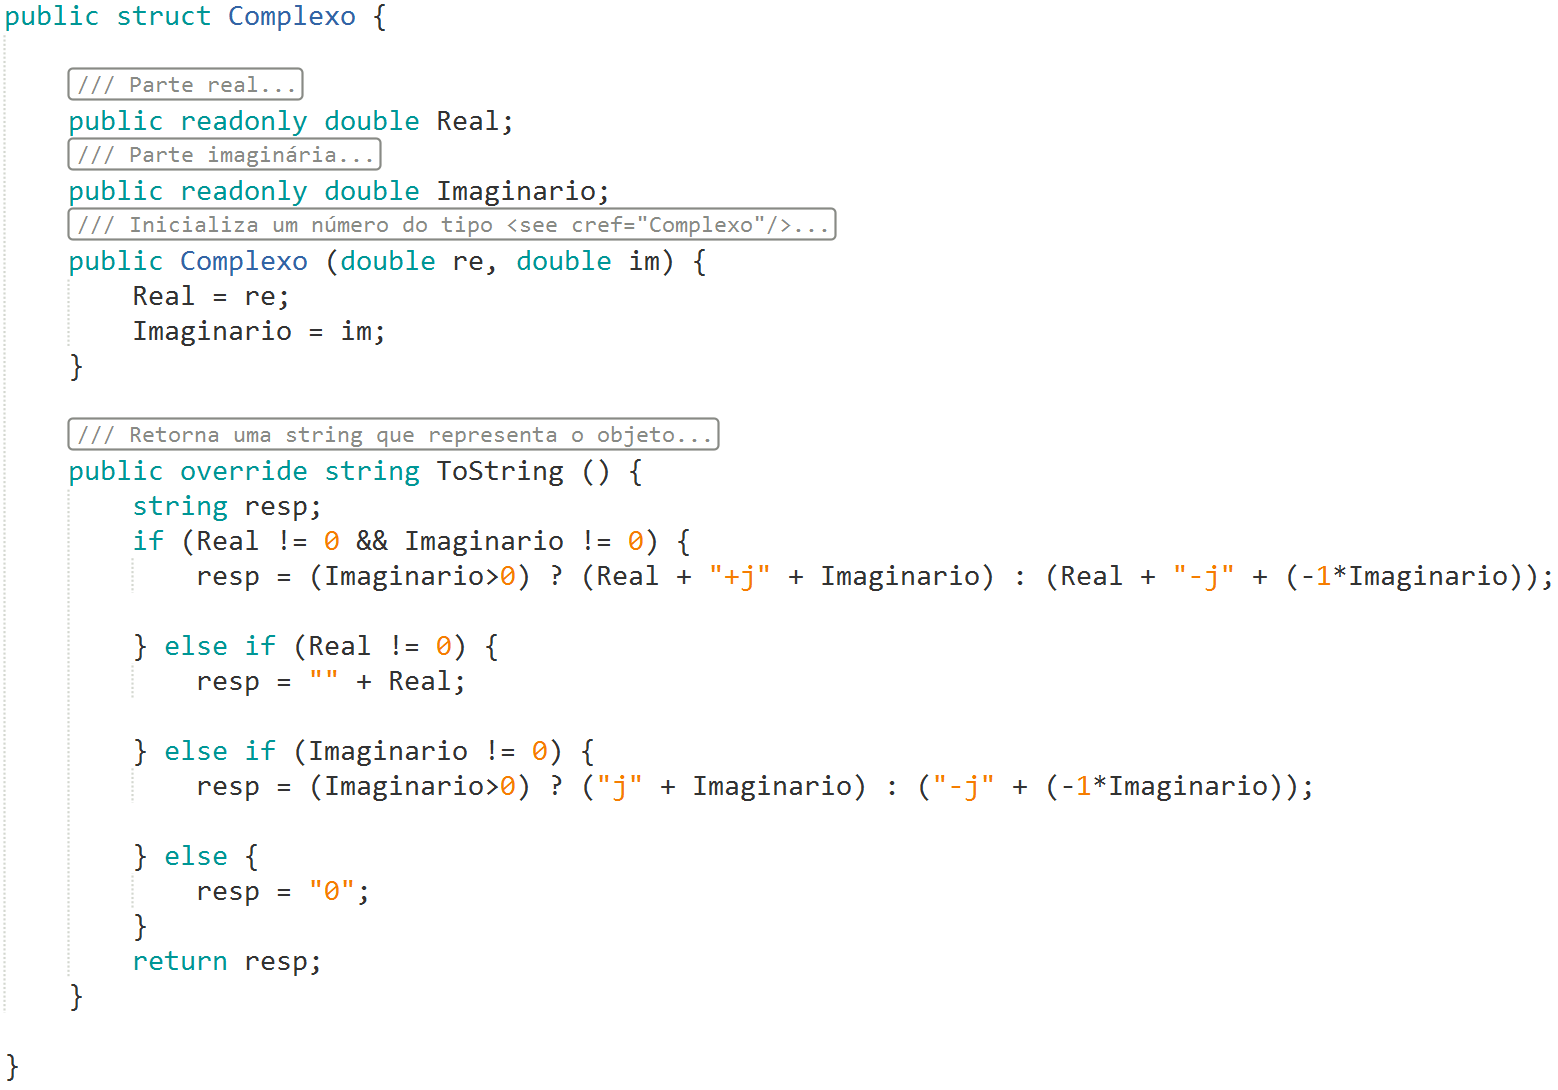
\includegraphics[width=\columnwidth]{complexo}
		\caption{Implementação da {\em struct} Complexo}
		\label{fig:complexo}
	\end{figure}
	
	\subparagraph{Fasor}A {\em struct} Fasor já é bem maior. Com 171 linhas incluindo documentação, essa struct é a responsável por toda e qualquer operação aritmética envolvendo fasores (figuras \ref{fig:fasor_op_1} e \ref{fig:fasor_op_2}) e pela geração de strings para cada representação existente (figuras \ref{fig:fasor_str_1} e \ref{fig:fasor_str_2}). O protótipo da struct pode ser encontrado na figura \ref{fig:fasor_prot}.
	\begin{figure}[h]
		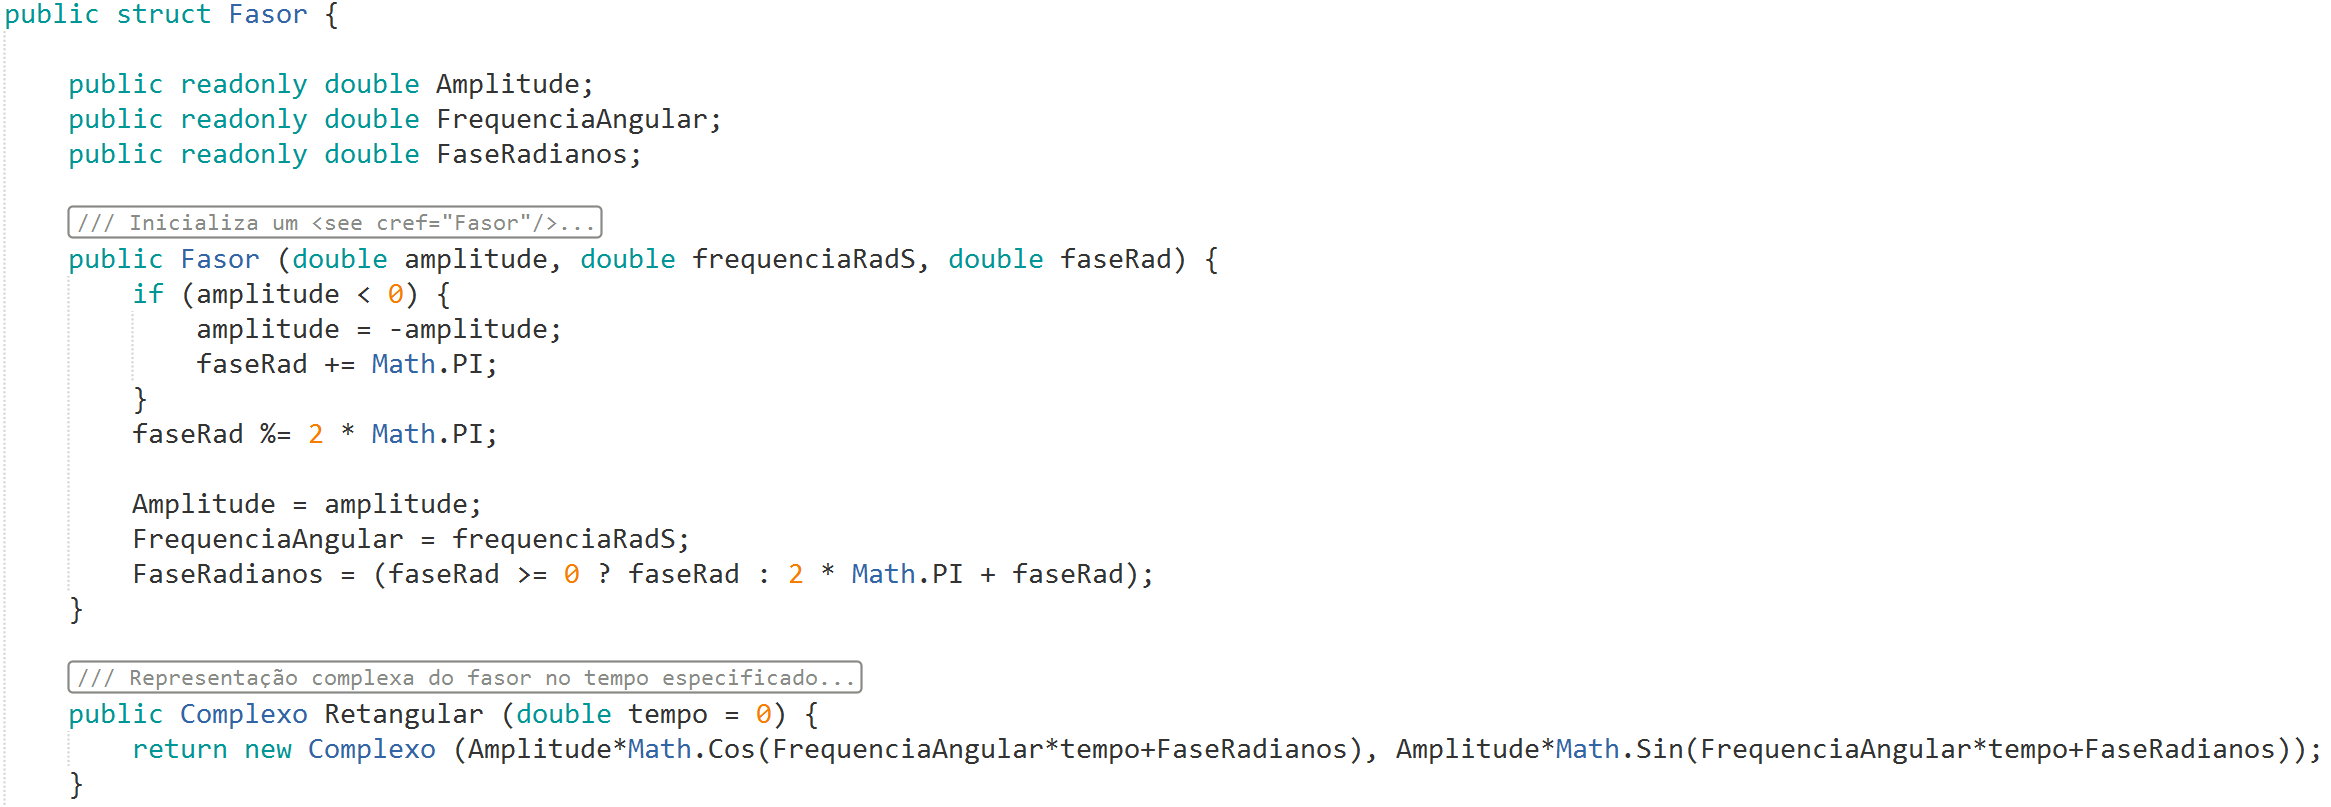
\includegraphics[width=\columnwidth]{fasor_1}
		\caption{Protótipo de Fasor}
		\label{fig:fasor_prot}
	\end{figure}
	
	Essa {\em struct} foi implementada com base na parte teórica deste relatório. Todas as funções e contas foram simplesmente uma implementação das equações da seção \ref{sec:arit}.
	
	Por exemplo, a operação de adição ({\em operator +} na imagem \ref{fig:fasor_op_1}) usa a equação \ref{eq:add}. A operação de subtração ({\em operator - (lhs, rhs)} na imagem \ref{fig:fasor_op_1}) usa a adição com o oposto ({\em operator - (lhs)} na imagem \ref{fig:fasor_op_1}) do segundo termo da operação, \ref{eq:sub}.
	A operação de multiplicação  ({\em operator * (lhs, rhs)} na imagem \ref{fig:fasor_op_1}) usa a equação \ref{eq:mult}. A operação de divisão ({\em operator / (lhs, rhs)} na imagem \ref{fig:fasor_op_1}) usa a multiplicação com o inverso ({\em Inverso} na imagem \ref{fig:fasor_op_1})  do segundo termo da operação, \ref{eq:div}.
	\begin{figure}[h]
		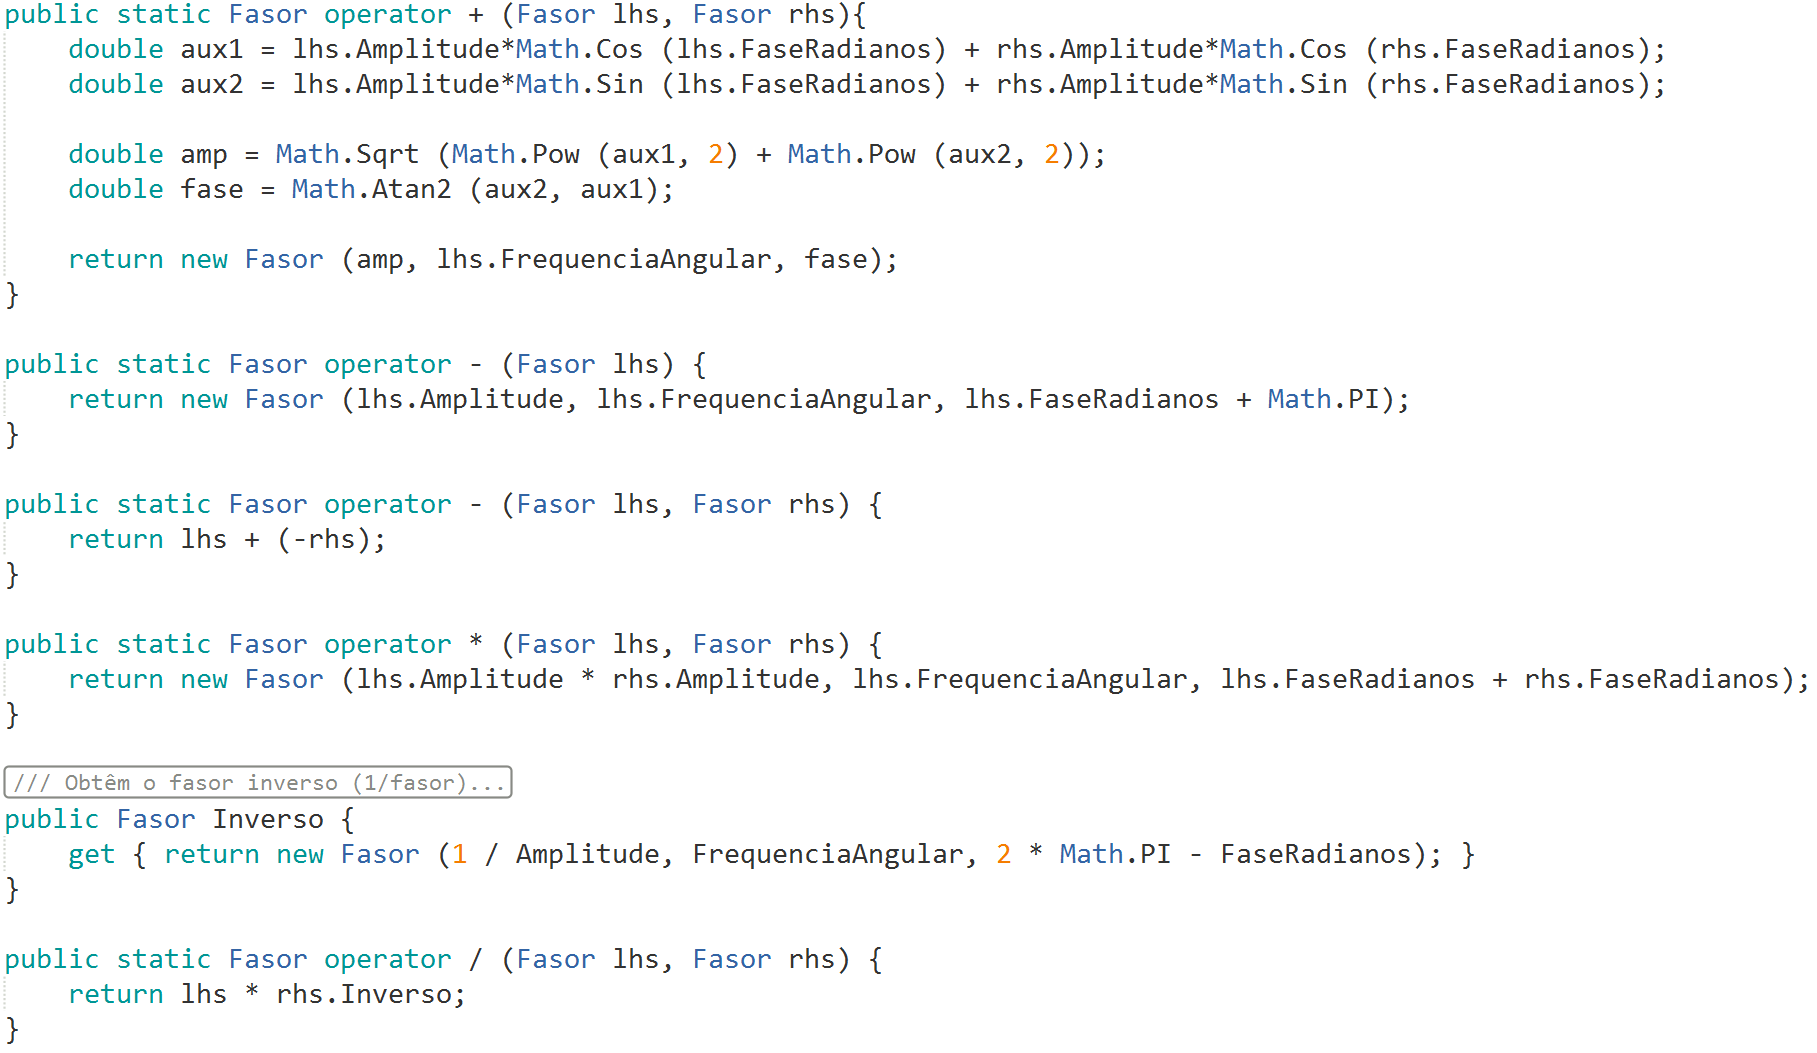
\includegraphics[width=\columnwidth]{fasor_4}
		\caption{Operações aritméticas}
		\label{fig:fasor_op_1}
	\end{figure}
	
	A operação conjugado complexo ({\em Conjugado} na imagem \ref{fig:fasor_op_2}) usa a equação \ref{eq:conj}. A operação de derivação ({\em Derivado} na imagem \ref{fig:fasor_op_2}) usa a equação \ref{eq:der}. E a operação de integração ({\em Integrado} na imagem \ref{fig:fasor_op_2}) usa a equação \ref{eq:int}.
	\begin{figure}[h]
		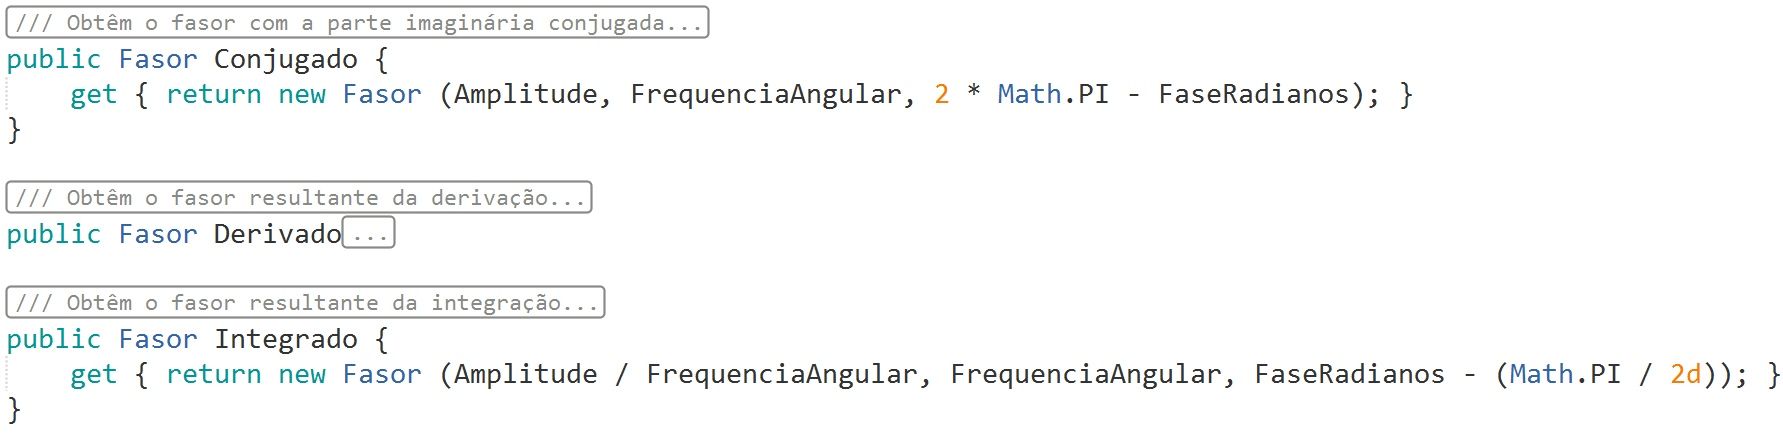
\includegraphics[width=\columnwidth]{fasor_5}
		\caption{Operações aritméticas}
		\label{fig:fasor_op_2}
	\end{figure}
	
	Com essas duas classes implementadas, a aplicação já pode ser construída da forma que se desejar e usando a ferramenta que quiser. Poderia ser OpenGL, WebGL, somente texto, Vulkan, Visual C\#, ou qualquer outra API gráfica existente no mercado. Como desejo fazer o código uma vez e fazer a entrega de executáveis em várias plataformas ao mesmo tempo, sem me preocupar com otimizações, para esse protótipo, decidi utilizar a ferramenta Unity. A partir da próxima seção será abordado os específicos de como foi executada a implementação com essa ferramenta.
	\begin{figure}[h]
		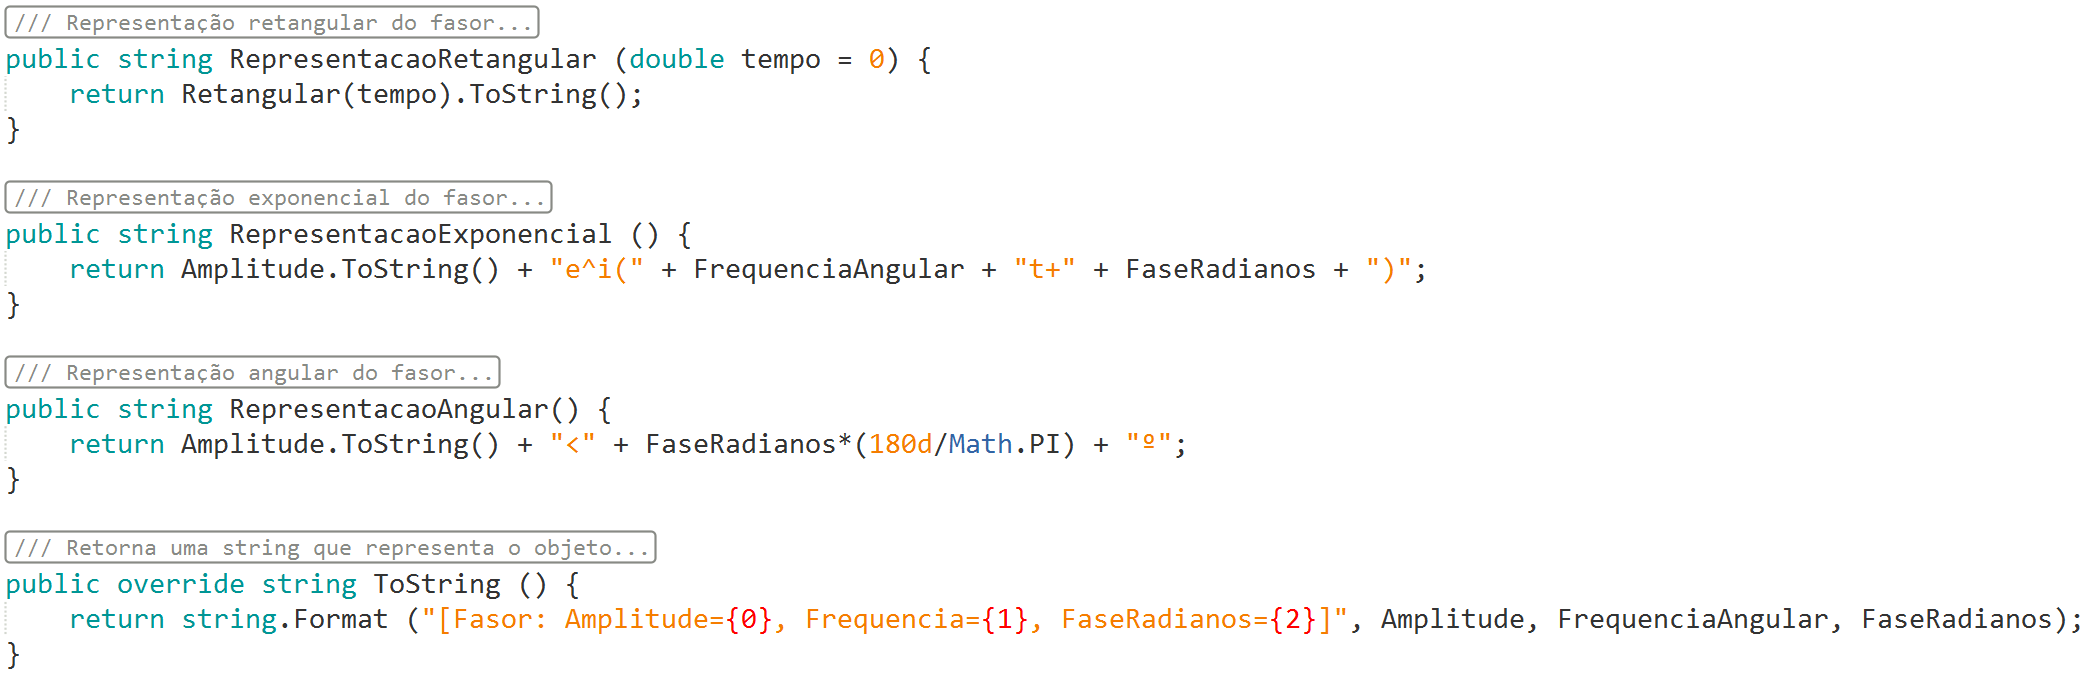
\includegraphics[width=\columnwidth]{fasor_3}
		\caption{Diversas representações por string}
		\label{fig:fasor_str_2}
	\end{figure}
	\begin{figure}[h]
		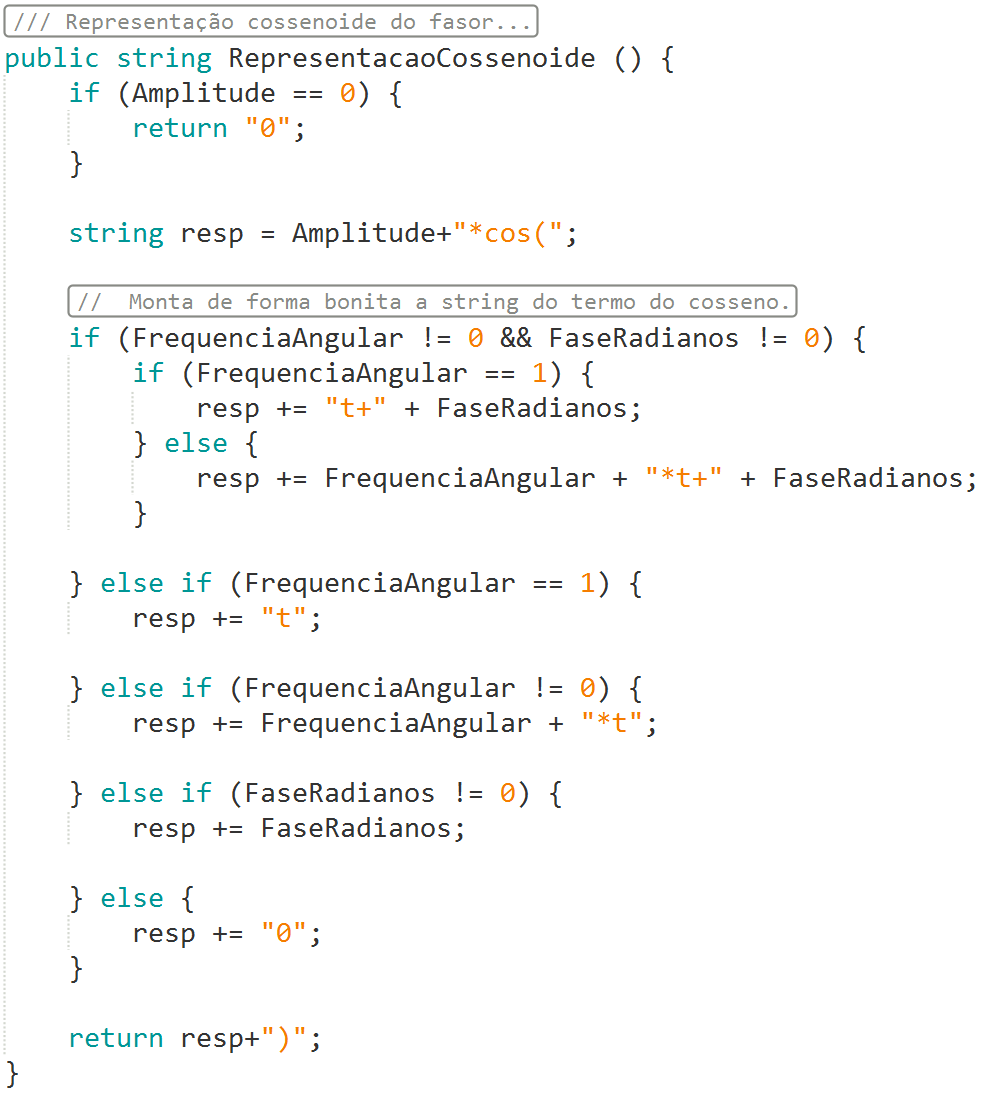
\includegraphics[width=\columnwidth]{fasor_2}
		\caption{Diversas representações por string}
		\label{fig:fasor_str_1}
	\end{figure}
	
	\subsection{Testes}
	\paragraph{}Primeiramente, para garantir o bom funcionamento da parte mateática, foram implementados testes unitários. Esses testes puderam assegurar a integridade dos resultados durante sua implementação. Quanto a parte gráfica, não foram criados testes unitários pois eles mais dependem de testes, tentativas e erros, ao usar a interface.
	
	\subsection{Arquitetura}
	\paragraph{}Como esse projeto foi proposto para ser feito em pouco tempo, somente um protótipo era planejado para o final. Portanto, a arquitura executada pode não ser a mais eficiente.
	
	Nesse projeto, a interface gráfica é que controla tudo. É a interface gráfica que possui gerentes de fasores, que decide quando mudar de tela e quando fazer as contas.
	
	Existem 3 cenas: Menu Principal, Visualização Fasorial e Cálculo Fasorial. Cada vez que se sai de uma cena, ao se retornar para ela, tudo será resetado. Da cena Menu Principal é possível ir para qualquer uma das outras cenas, mas cada cena só pode retornar para a cena principal.
	\subparagraph{Menu Principal}Nessa cena, existem dois botões. Cada um te permite ir para cada uma das outras duas cenas. Ela existe para pré-carregar recursos necessários e permitir o usuário decidir o que ele deseja fazer.
	\subparagraph{Visualização Fasorial}Em Visualização Fasorial, existe um menu-gaveta na parte de baixo da cena. Esse menu-gaveta é onde o usuário pode inserir ou remover fasores que serão mandados para a visualização no plano. Cada botão possui uma variável do tipo fasor que é onde é armazenado qual fasor aquele botão representa. É a função da classe responsável por desenhar no plano que pega esse fasor, obtêm o complexo no instante 0 e o plota no plano Real x Imaginário.
	\subparagraph{Cálculo Fasorial}Essa cena é a calculadora propriamente dita. É aqui que o usuário pode executar a operação que desejar. Como esse projeto está em fase de protótipo, só é possível fazer contas entre dois fasores e que possuem frequência angular iguais. Nesse caso, cada campo de inserção de dados é que possui um fasor e toda vez que um deles é terminado de ser editado, uma função é chamada que realiza a atualização do fasor resposta.

%	\bibliography{bibliografia}

\end{document}